\documentclass{beamer}
\usepackage{smartdiagram}
\mode<presentation> {
\usetheme{Madrid}
\setbeamertemplate{footline}[page number] % To replace the footer line in all slides with a simple slide count uncomment this line
}
\setbeamertemplate{bibliography item}{\insertbiblabel}
\usepackage{mathtools}
\usepackage{graphicx} % Allows including images
\usepackage{booktabs} % Allows the use of \toprule, \midrule and \bottomrule in tables
\usepackage{hyperref}
\hypersetup{
    colorlinks=true,
    linkcolor=blue,
    filecolor=magenta,      
    urlcolor=cyan,
}
\usepackage{url}


\title{Real-Time Control Methodologies \\ Using Open-Source Tools} 
\author{Sudhakar Kumar (183236001)} % Your name
\institute{

\includegraphics[scale=0.12]{images/iitb1.png} 
}
\date{\today} % Date, can be changed to a custom date

\begin{document}

\begin{frame}
\titlepage % Print the title page as the first slide
\end{frame}

\begin{frame}
\frametitle{Outline} 
\tableofcontents % Throughout your presentation, if you choose to use \section{} and \subsection{} commands, these will automatically be printed on this slide as an overview of your presentation
\end{frame}

\section{Motivation of the Study} 

\begin{frame}
\frametitle{Motivation of the Study}
In the post-PC era, an individual is interacting with several computers (or mini-computers) in his/her day-to-day activities. Most of these computers, which individuals are interacting with, fall under the umbrella of embedded real-time systems (ERTS). \\~\\

The reasons which can be attributed to the phenomenal proliferation of ERTS in day-to-day life are 
\begin{itemize}
    \item Reductions in the size and the cost of the computers
    \item Manifolds improvement in the performance 
    \item Increment in the processing power 
\end{itemize}
\vspace{0.4cm}
ERTSs are associated with various constraints like duration, delay, deadline, etc. Thus, there is a need to study the tools/algorithms which facilitate real-time sensing and control systems. 
\end{frame}
%------------------------------------------------

\section{What are Real-Time Systems?}
\begin{frame}
\frametitle{What are Real-Time Systems?}
Real-Time System (RTS) is an information processing system which has to respond to externally generated input stimuli within a finite and specified timing constraint. An RTS changes its state as a function of physical time. In these systems,
\begin{itemize}
    \item Correctness of the system behavior depends not only on the logical results of the computations, but also on the physical instant at which these results are produced.
    \item Failure to respond in time is as bad as the wrong response!
\end{itemize}
\vspace{0.4cm}
RTSs have a deadline before which it should respond. When our deadlines are big enough, pretty much any operating system will do.
\end{frame}
 
%------------------------------------------------

\begin{frame}{Applications of Real-Time Systems}
\textbf{Chemical Plant Control}: In an automated chemical plant, a real-time computer is deployed to periodically monitor the plant conditions. 
\begin{figure}[h]
    \centering
    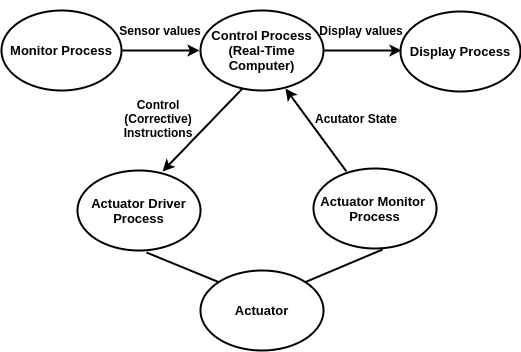
\includegraphics[width=0.75\textwidth]{images/chem.png}
    \caption{Flowchart for Real-Time Systems in an Automated Chemical Plant}
\end{figure}
\end{frame}

\begin{frame}{Applications of Real-Time Systems}
\textbf{Automated Car Assembly Plant}: At each workstation,
a sensor senses the arrival of the next partially assembled product. As soon as the partially assembled product is sensed, the workstation begins to execute its work on the work product.
\begin{figure}[h]
    \centering
    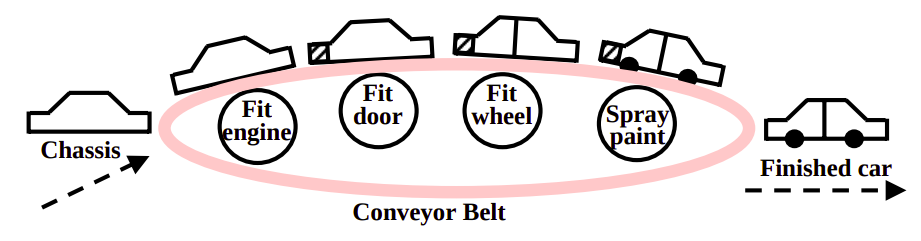
\includegraphics[width=0.75\textwidth]{images/car-assembly.png}
    \caption{Schematic Representation of an Automated Car Assembly Plant}
\end{figure}
\end{frame}

\begin{frame}{Applications of Real-Time Systems}
\textbf{Missile Guidance System}: A guided missile is capable of sensing an intended target and strikes it. Once the target is sensed
and detected, the missile needs to follow a trajectory to strike the target. \\~\\
\textbf{Computer On-board an Aircraft}: In modern aircrafts, a pilot can opt for auto pilot mode while flying aircraft. In this mode, an on-board computer takes over all controls of the aircraft including navigation, take-off, and landing of the aircraft. 
\begin{table}
\centering
\begin{tabular}{|c|c|}
 \hline
 \textbf{Applications} & \textbf{Time bound} \\
 \hline \hline
 Chemical plant control & few microseconds to several milliseconds \\ 
 \hline
 Automated car assembly plant & few hundreds of milliseconds\\ 
 \hline
 Missile guidance system & few hundreds of microseconds\\ 
 \hline
 Computer on-board an aircraft & few microseconds \\
 \hline
\end{tabular}
\caption{Applications of Real-Time Systems with its Time Bound}
\end{table}
\end{frame}

\begin{frame}{Basic Model of a Real-Time System}
\begin{figure}[h]
    \centering
    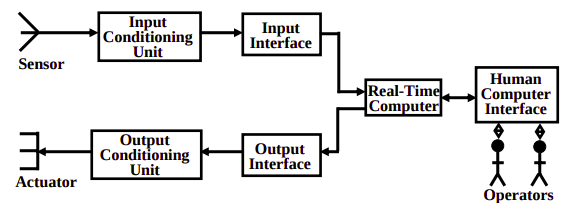
\includegraphics[width=\textwidth]{images/model-rts.png}
    \caption{Model of a Real-Time System}
\end{figure}
\end{frame}

\begin{frame}{Characteristics of Real-Time Systems}
    \begin{itemize}
        \item \textbf{Time constraints}: Every real-time task is associated with some time constraints. Therefore, the onus is on the RTS to ensure that all tasks meet their respective time constraints. 
        \item \textbf{Correctness Criterion}: In an RTS, correctness implies not only logical correctness of the results, but also the time at which the results are produced is of utmost importance.
        \item \textbf{Concurrency}: An RTS usually needs to respond to several independent events within very short and strict time bounds. 
        \item \textbf{Reactive}: RTSs are often reactive. A reactive system is one in which an ongoing interaction between the computer and the environment is maintained.
    \end{itemize}
Some other important characteristics include \textbf{stability}, \textbf{exception handling}, \textbf{custom hardware}, etc. 
\end{frame}

\begin{frame}{Classification of Real-Time Systems}
\textbf{Hard Real-Time Tasks}: The system is considered to have failed whenever any of its hard real-time tasks does not produce its required results before the specified time bound.\\
\textbf{Firm Real-Time Tasks}: Unlike a hard real-time task, even when a firm real-time task does not complete within its deadline, the system is not considered to have failed. \\
\textbf{Soft Real-Time Tasks}: The constraints are expressed either in terms of the average response times required. 
\begin{figure}[h]
\begin{tabular}{ll}
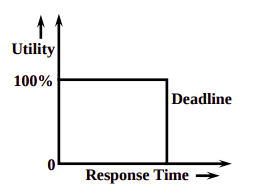
\includegraphics[scale=0.45]{images/firm-rts.png}
&
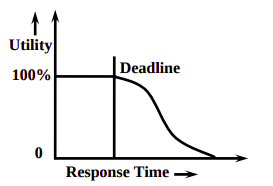
\includegraphics[scale=0.45]{images/soft-rts.png}
\end{tabular}
\caption{Left:  Utility of Result of a Firm Real-Time Task with Time. 
Right:  Utility of Result of a Soft Real-Time Task with Time}
\end{figure}
    
\end{frame}

\section{Types of Real-Time Tasks} 
\begin{frame}{Types of Real-Time Tasks} 
\textbf{Periodic Task}: One that repeats after a certain fixed time interval.
\begin{figure}[h]
    \centering
    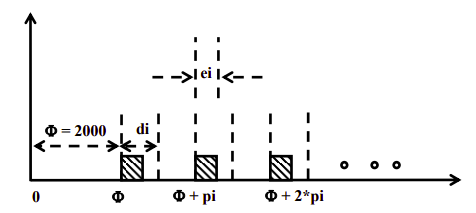
\includegraphics[width=0.75\textwidth]{images/periodic-task.png}
    \caption{Example of a Periodic Task (Track Correction Task of a Rocket)}
\end{figure}
For this task, phase = 2000 msec (occurrence of the first instance of the task), period = $p_i$, execution time = $e_i$, deadline = $d_i$. This task can be represented in a tuple as \fbox{$\tau_i = (\phi_i, p_i, e_i, d_i)$}. 
\end{frame}

\begin{frame}{Types of Real-Time Tasks}
    A vast majority of the tasks present in a typical real-time system are periodic. The reason for this is that many activities carried out by real-time systems are periodic in nature, e.g., monitoring certain conditions (as in a chemical plant). \\~\\
    \textbf{Sporadic Task}: One that recurs at random instants and has hard deadline e.g., I/O interrupt or DMA interrupt. It can be represented as \fbox{$\tau_i = (e_i, g_i, d_i)$}, where $g_i$ is the minimum separation between two consecutive instances of the task. \\~\\
    \textbf{Aperiodic Task}: Here, the minimum separation $g_i$ between two consecutive instances can be 0. That is, two or more instances of an aperiodic task might occur at the same time instant. The deadline for an aperiodic task is expressed as an average value. These tasks are generally soft real-time tasks, e.g.,  operator requests, keyboard presses, mouse movements, etc..
\end{frame}


\section{Real-Time Task Scheduling} 
\begin{frame}{Real-Time Task Scheduling}
\textbf{Clock-Driven (Static/Offline) Scheduling}:  These schedulers make their scheduling decisions (regarding which task to run next) only at the clock interrupt points. These schedulers fix the schedule before the system starts to run.  \\~\\
Let us consider four independent periodic tasks $\tau_1 = (p_i = 4, e_i = 1)$, $\tau_2 = (5, 1.8)$, $\tau_3 = (20, 1)$, and $\tau_4 = (20, 2)$. The  utilization $U =  \sum_{i=1}^{n} \frac{e_i}{p_i} = \frac{1}{4} + \frac{1.8}{5} + \frac{1}{20} + \frac{2}{20} = 0.76 < 1$. \\~\\
For this set of tasks, one possible schedule might be as given below: 
\begin{figure}[h]
    \centering
    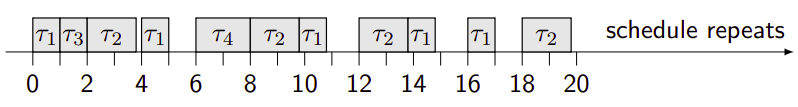
\includegraphics[width=\textwidth]{images/cyclic.png}
    \caption{Pre-Computed Schedule for four independent well-known Tasks}
\end{figure}
\end{frame}

\begin{frame}{Real-Time Task Scheduling}
\textbf{Event-Driven Scheduling}: Unlike cyclic schedulers, event-driven schedulers can handle aperiodic and sporadic tasks
more proficiently. However, these schedulers are less efficient as they deploy more complex scheduling algorithms and are are less suitable for embedded applications as these are required to be of small size, low cost, and consume minimal amount of power. 

\begin{table}[h]
\begin{tabular}{|c|c|c|}
 \hline
 \textbf{Parameter} &  \textbf{Clock-Driven} & \textbf{Event-Driven}\\
 \hline  \hline
 Design & Simple \& efficient & More sophisticated \\
 \hline
 Tasks & Periodic & Sporadic, aperiodic, periodic \\
 \hline
 Applications & Embedded systems &  Moderate and
large-sized applications \\ 
 \hline
 Scheduling & Offline & Online \\
 \hline
\end{tabular}
\caption{Comparison of Clock-Driven Scheduling and Event-Driven Scheduling}
\end{table}
\end{frame}

\section{Dynamic Scheduling}
\begin{frame}{Dynamic Scheduling}
\textbf{Deferrable Scheduling with Least Actual Laxity First (DS-LALF)}: In real-time sensing and control systems, there is a need to monitor the Quality of Data (QoD) along with the Quality of Control (QoC). There will always be a trade-off between maintaining the quality of real-time data objects and fulfilling the deadline constraints
of control transactions while ensuring both QoD and QoC.\\~\\

DS-LALF is proposed in \cite{ds-lalf} to maintain the validity of real-time data objects. In this algorithm, control transactions are assigned lower priorities compared with the update transactions. Thus, it will maximize the QoD while affecting the schedulability of control transactions. An extension of the algorithm DS-LALF, named Co-LALF is presented to resolve the coscheduling problem between update and control transactions in a real-time sensing and control
system. 
\end{frame}

\begin{frame}{Model of Co-LALF}
\begin{figure}[h]
    \centering
    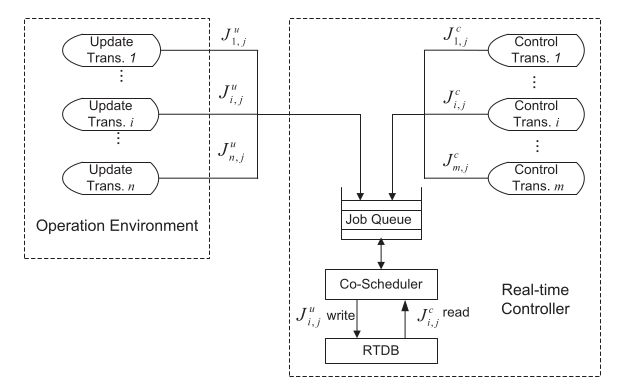
\includegraphics[width=0.88\textwidth]{images/ds-lalf.png}
    \caption{Conceptual System model of Co-LALF}
\end{figure}
\end{frame}

\begin{frame}{Dynamic Scheduling}
\textbf{Improving QoC using Flexible Timing Constraints}: A controller with flexible timing constraints is presented in \cite{qoc} which allows the design of discrete-time controllers depending upon a finite set of values for the sampling period and on a finite set of values for the time delay.  \\~\\

By selecting specific EXAST (EXAct start time Separation constrainT) and  EXACT (EXAct start-to-Completion time-interval constrainT) values, the control task instance execution can be enabled to adapt according to the system dynamics. It means that when the controlled system response deviates due to perturbations, we will be able to speed up the execution of the controller in order to minimize such deviations, and when perturbations are not affecting the system, we can slow down the controller execution rate in order to save resources.
\end{frame}

\section{Unix as an RTOS}
\begin{frame}{Unix as an RTOS}
The traditional Unix operating system suffers from several
shortcomings when used in real-time applications, as given below: 
\begin{itemize}
    \item \textbf{Non-Preemptive Kernel}: A process running in kernel mode cannot be preempted by other processes i.e., the Unix kernel is non-preemptive. On the other hand, the Unix system does preempt processes running in the user mode. As a consequence, even when a low priority process makes a system call, the high priority processes would have to wait until the system call completes. 
    \item \textbf{Dynamic Priority Levels}: In Unix systems, real-time tasks can not be assigned static priority values. This is due to the fact that the operating system alters the priority value, after a programmer sets it. This makes it very difficult to schedule real-time tasks. 
\end{itemize}
\end{frame}

\section{Windows as an RTOS}
\begin{frame}{Windows as an RTOS}
Windows NT has several features which are very desirable for real-time applications such as support for multi-threading, real-time priority levels, and timer. Moreover, the clock resolutions are sufficiently fine for most real-time applications. \\~\\

In spite of the impressive support that Windows provides for real-time program development, it is neither advisable nor feasible to use NT for hard real-time applications, for example, at the controller level with sub-millisecond precision as pointed out in \cite{windowsnt-k}. 
\end{frame}

\section{Tools for enabling Real-Time Features}
\begin{frame}{Tools for enabling Real-Time Features}
\textbf{Linux as an RTS}: RT Linux, and RTAI.\\
\textbf{RT Linux}: RT Linux runs along with a Linux system. The real-time kernel sits between the hardware and the Linux system. The RT kernel intercepts all interrupts generated by the hardware. If an interrupt is to cause a real-time task to run, the real-time kernel preempts Linux, if Linux is running at that time, and lets the real-time task run. Thus, in effect Linux runs as a task of RT Linux.
\begin{figure}[h]
    \centering
    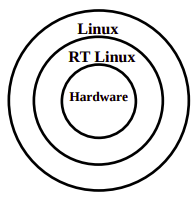
\includegraphics[width=0.3\textwidth]{images/rtlinux.png}
    \caption{Structure of RT Linux}
\end{figure}
\end{frame}

\begin{frame}{RealTime Application Interface (RTAI) for Linux}
RTAI provides a more practical API while RT Linux is more elegant. The RTAI team makes a constant effort to add features that people ask for. For instance, RTAI includes clock (8254 and APIC) calibration, dynamic memory management for real-time tasks, LXRT (Linux Extension for Real-Time) to bring soft/hard real-time capabilities into user space, remote procedure calls, and mailboxes. \\~\\

Due to the practicality of RTAI API, an open source project named RTAI-Lab aims to provide a common structure framework for the integration of RTAI into the Scilab environment, as mentioned in \cite{scilab-rtai}. 
\end{frame}

\begin{frame}{Simulation Flags in OpenModelica}
\begin{figure}[h]
    \centering
    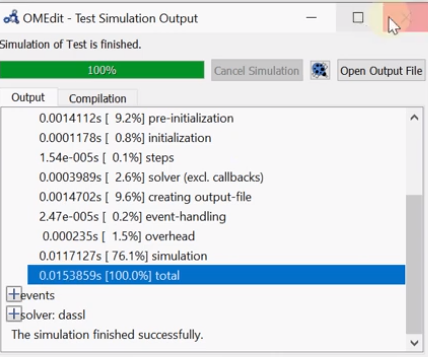
\includegraphics[width=0.68\textwidth]{images/without-rt.png}
    \caption{Simulating without Real-Time Flag in OpenModelica}
\end{figure}
\end{frame}

\begin{frame}{Simulation Flags in OpenModelica}
\begin{figure}[h]
    \centering
    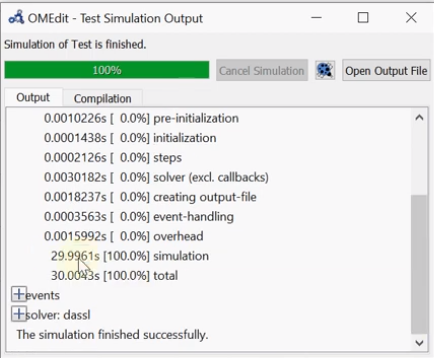
\includegraphics[width=0.68\textwidth]{images/with-rt.png}
    \caption{Simulating with Real-Time Flag in OpenModelica}
\end{figure}
\end{frame}

\begin{frame}{FreeRTOS Task Implementation in Arduino IDE}
\begin{itemize}
    \item Blink an LED at digital pin 8 with 200ms frequency.
    \item Blink another LED digital pin 7 with 300ms frequency.
    \item Print numbers in serial monitor with 500ms frequency. 
\end{itemize}

\begin{figure}[h]
\centering
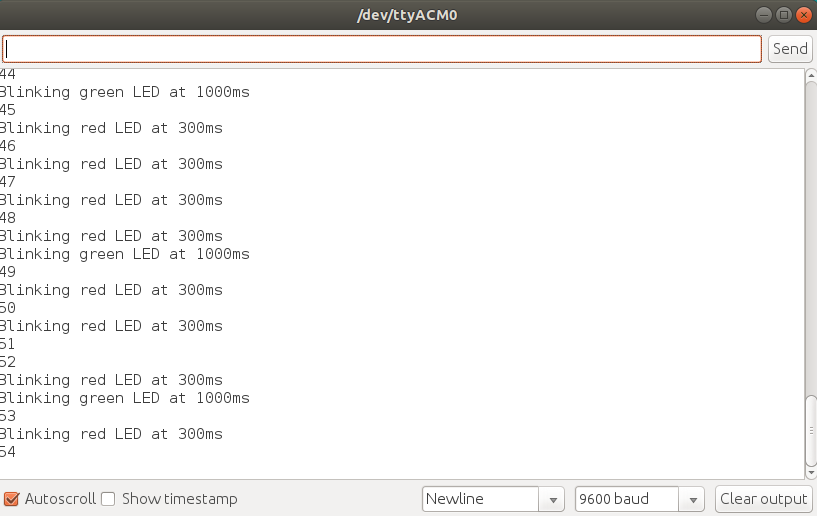
\includegraphics[width=0.75\textwidth]{images/Arduino-ide-tasks.png}
\caption{Serial Monitor of Arduino IDE with the Tasks (being executed)}
\end{figure}
\end{frame}

\section{Conclusion}
\begin{frame}{Conclusion}
\begin{itemize}
    \item For non-real-time tasks, the associated time bounds are typically of the order of a few minutes, hours or even days. In contrast, the time bounds associated with soft real-time tasks are at most of the order of a few seconds.
    \item The tools like RTLinux, RTAI, etc can be deployed to make Linux into a real-time system. 
    \item Real-time flags in OpenModelica and FreeRTOS in Arduino can be deployed for real-time synchronization and multitasking. 
\end{itemize}
    
\end{frame}

\section{References}
\begin{frame}{References}
\begin{thebibliography}{111}
    \bibitem{ds-lalf}
    \footnotesize{S. Han, K. Lam, J. Wang, K. Ramamritham and A. K. Mok, ``On Co-Scheduling of Update and Control Transactions in Real-Time Sensing and Control Systems: Algorithms, Analysis, and Performance," in IEEE Transactions on Knowledge and Data Engineering, vol. 25, no. 10, pp. 2325-2342, Oct. 2013, doi: 10.1109/TKDE.2012.173.}
    
    \bibitem{qoc}
    P. Marti, J. M. Fuertes, G. Fohler and K. Ramamritham, ``Improving quality-of-control using flexible timing constraints: metric and scheduling," 23rd IEEE Real-Time Systems Symposium, 2002. RTSS 2002., Austin, Texas, USA, 2002, pp. 91-100, doi: 10.1109/REAL.2002.1181565.
    
    \bibitem{windowsnt-k}
    K. Ramamritham, ``Can real-time systems be built from off-the-shelf components?," Proceedings Sixth International Conference on Real-Time Computing Systems and Applications. RTCSA'99 (Cat. No.PR00306), Hong Kong, China, 1999, pp. 226-226, doi: 10.1109/RTCSA.1999.811233.
    
    \bibitem{scilab-rtai}
    C. Meza, J. A. Andrade-Romero, R. Bucher and S. Balemi, ``Free open source software in control engineering education: A case study in the analysis and control design of a rotary inverted pendulum," 2009 IEEE Conference on Emerging Technologies \& Factory Automation, Mallorca, 2009, pp. 1-8, doi: 10.1109/ETFA.2009.5347162.

\end{thebibliography}
\end{frame}


\end{document}
